\documentclass[final,5p,times,twocolumn]{elsarticle}

\usepackage{graphicx}  %% For figures
\usepackage{lipsum}     %% For placeholder text
\usepackage{comment}    %% For long text comments
\usepackage{amsmath}    %% For equations
\usepackage{longtable}
\usepackage{amsmath, amssymb}
\usepackage{subcaption}
\usepackage{bbm}
\usepackage{ulem}
\usepackage{pgfplotstable}
\pgfplotsset{compat=1.17}
\usepackage{tabularx}    % Tabelle a larghezza automatica
\usepackage{booktabs}    % Migliore stile di tabelle (toprule, midrule, bottomrule)
\usepackage{adjustbox}   % Per limitare larghezza (max width)
\usepackage[hidelinks]{hyperref}

%% Define custom commands
\newcommand{\kms}{km\,s$^{-1}$}
\newcommand{\msun}{$M_\odot$}

%% Journal name placeholder
\journal{}

\makeatletter
\def\ps@pprintTitle{%
 \let\@oddhead\@empty
 \let\@evenhead\@empty
 \let\@oddfoot\@empty
 \let\@evenfoot\@empty
}
\makeatother

\begin{document}

\begin{frontmatter}

\title{%
  \small\textsc{Università degli Studi di Salerno\\
  Corso di Laurea Magistrale in Informatica (LM-18)\\
  Intelligenza Artificiale, coorte 2025/2026 \\
  prof. Vincenzo Deufemia} \\[4pt]
  \Large Generazione Automatica di Videogiochi tramite VGDL: \\
  Un Approccio Basato su Large Language Model e Reinforcement Learning
}

%% Author information
\author{Mattia Maucioni$^1$, Antonio Landi$^1$}

\address{$^1$Track: Data Science \& Machine Learning}

\begin{abstract}
La generazione automatica di videogiochi rappresenta una sfida all'avanguardia all'intersezione tra intelligenza artificiale e generazione procedurale di contenuti. Questo lavoro indaga l'utilizzo di Large Language Model (LLM) per la generazione automatica di codice nel Video Game Description Language (VGDL), un formalismo testuale di alto livello per la descrizione di regole di gioco, interazioni tra sprite e condizioni di terminazione. Viene costruito un dataset dedicato composto da descrizioni di giochi in VGDL abbinate a corrispondenti spiegazioni in linguaggio naturale, derivate da repository open source esistenti. Vengono successivamente addestrati e valutati più LLM in tre condizioni sperimentali: inferenza zero-shot, fine-tuning supervisionato e raffinamento tramite Reinforcement Learning (RL). L'analisi comparativa tra queste condizioni consente di quantificare il contributo di ciascun paradigma di addestramento alla qualità del codice VGDL generato. Questo studio si propone di mettere in luce sia il potenziale che le attuali limitazioni degli approcci basati su LLM per la generazione formale di giochi, offrendo spunti sulle sfide legate all'applicazione dei moderni modelli linguistici a linguaggi formali specifici di dominio.
\end{abstract}


%%\begin{keyword}
%%\end{keyword}

\end{frontmatter}

\section{Introduzione}
La generazione procedurale di videogiochi è da tempo oggetto di interesse nella ricerca in intelligenza artificiale, motivata dal potenziale di automatizzare processi creativi, ridurre i costi di sviluppo e abilitare la prototipazione rapida di esperienze interattive.

Tra i formalismi proposti per rappresentare la logica di gioco in modo compatto e interpretabile, il Video Game Description Language (VGDL) \citep{6633610} si distingue come un framework particolarmente espressivo. Il VGDL consente agli sviluppatori di definire la struttura completa di un gioco attraverso una specifica testuale concisa, che comprende definizioni degli sprite, regole di interazione, mappature dei livelli e condizioni di terminazione. Questa compattezza lo rende un obiettivo naturale per i modelli generativi, poiché una descrizione VGDL semanticamente valida è sufficiente per istanziare un gioco pienamente funzionante all'interno di ambienti di simulazione compatibili come py-vgdl.

I recenti progressi nei Large Language Model hanno dimostrato capacità notevoli nei compiti di generazione di codice in un'ampia gamma di linguaggi di programmazione e formalismi specifici di dominio. Tuttavia, la loro applicazione a linguaggi altamente strutturati e semanticamente vincolati come il VGDL rimane in gran parte inesplorata. Generare codice VGDL valido a partire da descrizioni in linguaggio naturale richiede non solo correttezza sintattica, ma anche una comprensione profonda delle meccaniche di gioco, del comportamento degli sprite e della consistenza logica tra i componenti in interazione. 

Questo progetto affronta tale lacuna indagando sistematicamente la capacità degli LLM di generare codice VGDL in condizioni di addestramento progressivamente più informate. A partire da un dataset costruito da repository di giochi esistenti, in cui ogni gioco è annotato con una descrizione in linguaggio naturale che ne cattura regole, obiettivi e dinamiche, vengono valutati più LLM in un contesto zero-shot per stabilire una baseline. Si applica successivamente il fine-tuning supervisionato per esporre i modelli a pattern specifici del dominio, impiegando infine tecniche di Reinforcement Learning per allineare ulteriormente gli output generati a criteri di correttezza strutturale e funzionale.

I contributi che questo lavoro si propone di raggiungere sono quattro: la costruzione di un nuovo dataset VGDL che abbina descrizioni in linguaggio naturale al corrispondente codice di gioco; una valutazione comparativa di più LLM nelle configurazioni zero-shot, supervisionata e raffinata tramite RL; un'analisi dell'efficacia del fine-tuning supervisionato e dell'RL nel migliorare la qualità funzionale delle descrizioni di gioco generate; e una discussione delle principali sfide incontrate durante l'implementazione, dalla costruzione del dataset alla progettazione della funzione di reward.

% -------------------------------------------------------
\section{Costruzione del Dataset}
% -------------------------------------------------------

La disponibilità di un dataset è un prerequisito fondamentale per addestrare e valutare LLM nel dominio specifico del VGDL. Non esistendo, a nostra conoscenza, alcun dataset pubblicamente disponibile che abbini descrizioni in linguaggio naturale a codice VGDL corrispondente, il primo contributo di questo lavoro consiste nella sua costruzione da zero.

\subsection{Raccolta dei Dati Grezzi}

Il materiale grezzo è stato raccolto principalmente dal repository ufficiale di \texttt{py-vgdl} e da raccolte derivate accessibili su GitHub, le quali includono implementazioni di giochi arcade classici (Frogger, Aliens, Zelda, ecc.) e varianti originali sviluppate dalla comunità di ricerca GVGAI. In totale sono stati estratti 201 file \texttt{.vgdl}, ciascuno composto da due blocchi principali: la game description (definizione degli sprite e delle regole di interazione) e la level description (mappatura della griglia di gioco).

Per garantire la qualità dei campioni, ogni file è stato sottoposto a un processo di rimozione del level description e validazione automatica tramite il parser interno di \texttt{py-vgdl}.

\subsection{Generazione delle Descrizioni in Linguaggio Naturale tramite LLM}

La costruzione delle annotazioni testuali ha seguito un approccio automatico basato su prompt engineering. È stato progettato un prompt strutturato che, a partire dai blocchi VGDL analizzati, istruisce il modello Claude Sonnet 4.6 (Anthropic) interrogato tramite API a generare una descrizione in linguaggio naturale del gioco articolata secondo tre dimensioni: (i) gli attori presenti nella scena e le loro proprietà cinematiche, (ii) le regole di interazione tra sprite e (iii) le condizioni di terminazione con relativo esito (vittoria o sconfitta). 
Il modello ha generato iterativamente una descrizione per ciascuno dei 201 file VGDL raccolti. Le descrizioni prodotte sono state successivamente verificate per accertarne la correttezza semantica rispetto al codice sorgente corrispondente. 
Il risultato è un dataset di coppie ⟨codice VGDL, descrizione⟩ in cui il codice VGDL costituisce l'input del modello e il testo in linguaggio naturale rappresenta il target da generare.

\subsection{Suddivisione e Caratteristiche del Dataset}

Il dataset è stato suddiviso in due partizioni: insieme di addestramento (\textit{train}) e di test (\textit{test}). La partizione è stata eseguita in modo da garantire l'assenza di sovrapposizioni semantiche tra i due sottoinsiemi, evitando che varianti dello stesso gioco base finissero in insiemi diversi.

Il dataset, una volta consolidato, verrà reso pubblicamente disponibile per favorire la riproducibilità degli esperimenti e incoraggiare ricerche future in questo dominio.

\section{Selezione dei Modelli}

La scelta dei modelli da sottoporre a valutazione ha seguito criteri che bilanciano copertura dello spazio delle architetture disponibili, accessibilità per il fine-tuning e rilevanza rispetto allo stato dell'arte nella generazione di codice.

\subsection{Criteri di Selezione}

Sono stati adottati i seguenti criteri guida nella selezione:
\begin{itemize}
  \item \textbf{Capacità di generazione di codice}: preferenza per modelli pre-addestrati su dataset che includono codice sorgente, in quanto il VGDL condivide con i linguaggi di programmazione la necessità di rispettare una sintassi formale rigida.
  \item \textbf{Dimensione del modello}: bilanciamento tra modelli di dimensione ridotta (adatti al fine-tuning su hardware accessibile) e modelli di maggiori dimensioni (utili come baseline di riferimento in modalità zero-shot).
  \item \textbf{Disponibilità dei pesi}: preferenza per modelli open-weight che consentono il fine-tuning completo o tramite tecniche efficienti quali LoRA \citep{hu2022lora}.
\end{itemize}


\subsection{Modelli Impiegati}

In base ai criteri sopra enunciati, sono stati impiegati i seguenti modelli:

\paragraph{DeepSeek-LLM-7B-Chat} \citep{deepseek-llm} Modello decoder-only da 7 miliardi di parametri sviluppato da DeepSeek AI, addestrato su un ampio dataset bilingue (cinese e inglese) con enfasi sulla generazione di codice. La variante \textit{chat} è stata instruction-tuned per il dialogo ed il seguire istruzioni.

\paragraph{Qwen2.5-3B-Instruct} \citep{qwen2.5} Modello della famiglia Qwen 2.5 di Alibaba da 3 miliardi di parametri, ottimizzato per seguire istruzioni. Addestrato su un dataset esteso che include codice sorgente in diversi linguaggi di programmazione.

\paragraph{Qwen3.5-4B} \citep{qwen3.5} Modello della famiglia Qwen 3.5 di Alibaba da 4 miliardi di parametri, evoluzione della serie Qwen con miglioramenti nelle capacità di ragionamento e generazione di codice strutturato.

\paragraph{Mistral-7B-Instruct-v0.3} \citep{jiang2023mistral7b} Modello decoder-only da 7 miliardi di parametri di Mistral AI, basato su attention con sliding window. La versione \textit{instruct} è stata ottimizzata tramite RLHF per seguire istruzioni in linguaggio naturale.

\paragraph{Phi-3.5-mini-instruct} \citep{abdin2024phi3} Modello compatto da circa 3.8 miliardi di parametri sviluppato da Microsoft, progettato per ottenere prestazioni elevate con dimensioni ridotte attraverso un training su dati sintetici di alta qualità (\textit{textbooks-are-all-you-need}).

\paragraph{GPT-Neo-2.7B} \citep{gpt-neo} Modello autoregressive open-source da 2.7 miliardi di parametri sviluppato da EleutherAI come replica open della famiglia GPT. Addestrato sul dataset The Pile, rappresenta una baseline di riferimento per modelli di generazione testuale open-weight.

\paragraph{Minerva-7B-instruct-v1.0} \citep{orlando2024minerva} Modello da 7 miliardi di parametri sviluppato dal laboratorio Sapienza NLP dell'Università "La Sapienza" per la lingua italiana, basato sull'architettura LLaMA 2 e addestrato su un dataset italiano esteso. La variante \textit{instruct} è stata fine-tuned per seguire istruzioni in italiano.

\subsection{Protocollo di Valutazione Zero-Shot}

I modelli sono stati valutati in modalità zero-shot sulla capacità di generare codice VGDL a partire da una descrizione in linguaggio naturale del gioco, senza alcun esempio fornito nel prompt. La valutazione si articola su due dimensioni complementari.

La prima dimensione è l'\textbf{eseguibilità} del codice generato: il VGDL prodotto dal modello viene sottoposto al parser della libreria \texttt{py-vgdl}, che ne verifica la correttezza sintattica e strutturale. Un file VGDL viene considerato valido se il parser lo accetta senza errori.

La seconda dimensione è la \textbf{similarità strutturale} con il VGDL target, ovvero il codice originale da cui è stata derivata la descrizione in linguaggio naturale fornita al modello. La similarità è calcolata dal modulo \texttt{eval\_similarity.py} tramite indice di Jaccard applicato a tre componenti estratte dal codice VGDL: gli sprite foglia definiti nel \texttt{SpriteSet} (peso 0.25), le interazioni nell'\texttt{InteractionSet} (peso 0.50) e le condizioni di terminazione nel \texttt{TerminationSet} (peso 0.25). Il punteggio finale è la media pesata dei tre indici:
\[
  \text{sim} = 0.25 \cdot J_\text{sprite} + 0.50 \cdot J_\text{interaction} + 0.25 \cdot J_\text{termination}
\]
dove $J(A, B) = |A \cap B| / |A \cup B|$. L'indice delle interazioni riceve peso doppio in quanto cattura la logica di gioco, mentre sprite e condizioni di terminazione contribuiscono in egual misura come contorno strutturale.

\section{Fine-Tuning - Learning Supervisionato}

L'approccio zero-shot fornisce una prima indicazione delle capacità generative dei modelli selezionati, ma non sfrutta la disponibilità di esempi etichettati nel dataset costruito. Il passo successivo consiste nel fine-tuning supervisionato (SFT, \textit{Supervised Fine-Tuning}): il modello viene esposto a coppie \textit{(descrizione testuale, codice VGDL target)} e aggiornato per massimizzare la verosimiglianza del codice corretto dato l'input. In questo modo il modello acquisisce familiarità con la sintassi VGDL e con le convenzioni strutturali del dominio, che difficilmente emergono dal solo pre-addestramento su dataset generici.

\subsection{Tecnologie di Training Impiegate}

Addestrare un modello da miliardi di parametri nella sua interezza richiederebbe risorse computazionali proibitive. Per questo motivo si è fatto ricorso a due tecniche complementari di efficienza.

LoRA (\textit{Low-Rank Adaptation}) è una tecnica di adattamento efficiente dei parametri (PEFT) che, anziché aggiornare l'intera matrice dei pesi, inietta coppie di matrici a basso rango $\Delta W = BA$ nei layer selezionati dell'architettura. Il numero di parametri addestrabili si riduce drasticamente: il rango $r$ controlla il compromesso tra capacità espressiva e costo computazionale.

QLoRA \citep{dettmers2023qlora} estende LoRA quantizzando il modello base a 4 bit (formato NF4, \textit{NormalFloat4}), mantenendo le matrici LoRA in precisione piena durante il forward pass. Questo permette di caricare e addestrare modelli da diversi miliardi di parametri su una singola GPU consumer, con una perdita di qualità trascurabile rispetto al full fine-tuning.

Unsloth \citep{unsloth} è una libreria open-source che ottimizza l'esecuzione del training di LLM tramite kernel CUDA personalizzati e un'implementazione efficiente del gradient checkpointing. Rispetto a un training vanilla con Hugging Face \texttt{Trainer}, Unsloth riduce il consumo di memoria VRAM fino al 60\% e accelera il training fino a $2\times$, rendendo praticabile il fine-tuning su hardware accessibile.

\subsection{Fine-Tuning di Qwen3.5-4B}

Il primo modello sottoposto a fine-tuning supervisionato è Qwen3.5-4B, caricato in 4-bit tramite QLoRA via Unsloth. La configurazione LoRA adottata prevede rango $r=16$, $\alpha=32$ e dropout pari a $0.05$, applicata ai moduli di attenzione (\texttt{q\_proj}, \texttt{k\_proj}, \texttt{v\_proj}, \texttt{o\_proj}) e ai layer feed-forward (\texttt{gate\_proj}, \texttt{up\_proj}, \texttt{down\_proj}). Il training è stato eseguito per 5 epoche con learning rate $2 \times 10^{-4}$, scheduler cosine con 10 step di warmup e batch size effettivo pari a 8 (batch per dispositivo 2, gradient accumulation 4). L'ottimizzatore scelto è \texttt{paged\_adamw\_8bit}. L'intera sessione di training si è conclusa in circa 23 minuti su singola GPU.

\begin{figure}[h]
  \centering
  
\includegraphics[width=\columnwidth]{img/finetune/qwen35/training_loss_curve.png}
  \caption{Curve di loss per il fine-tuning di Qwen3.5-4B. In blu la training loss per step; in arancione la validation loss valutata al termine di ciascuna epoca. La linea tratteggiata indica il miglior checkpoint (step 115, eval loss $= 0.79$).}
  \label{fig:qwen35_loss}
\end{figure}

Come si osserva in Figura~\ref{fig:qwen35_loss}, la training loss cala rapidamente dai valori iniziali intorno a $2.007$ fino a $0.589$ al termine della terza epoca, con la maggior parte del progresso concentrata nella prima epoca. La validation loss segue un andamento coerente, passando da $0.916$ alla prima epoca a $0.749$ alla terza, corrispondente al miglior checkpoint salvato al passo 69. A partire da tale punto il modello non mostra ulteriori miglioramenti sulla validation, segnale evidente di overfitting. Il learning rate ha seguito uno scheduler cosine con warmup, raggiungendo il picco di $2.0 \times 10^{-4}$ intorno al passo 20 per poi decrescere fino a valori prossimi a zero al termine del training. La norma del gradiente oscilla nell'intervallo $[0.601, 0.779]$ senza tendenze crescenti, indicando un training numericamente stabile.

\subsection{Fine-Tuning di DeepSeek-LLM 7B}

Il secondo modello sottoposto a fine-tuning supervisionato è DeepSeek-LLM 7B Chat, un modello causale con circa 7 miliardi di parametri. A differenza del Qwen3.5-4B, per il quale la quantizzazione a 4 bit rappresentava una scelta orientata all'efficienza, nel caso del DeepSeek-LLM 7B essa si è rivelata una necessità imposta dai vincoli di memoria: caricando il modello in precisione \texttt{bfloat16} i soli pesi base richiederebbero oltre 14~GB di VRAM, superando la capacità disponibile. L'adozione di QLoRA con formato NF4 ha ridotto il footprint a circa 4~GB, rendendo praticabile il fine-tuning senza ricorrere a hardware dedicato di fascia alta.

La configurazione LoRA è identica a quella utilizzata precedentemente: rango $r = 16$, $\alpha = 32$, dropout $0.05$, applicata agli stessi moduli di attenzione e feed-forward. Il training si è svolto per 5 epoche con learning rate massima $2 \times 10^{-4}$, scheduler coseno con 10 step di warmup, batch size effettivo pari a 8 e ottimizzatore \texttt{paged\_adamw\_8bit}. L'intera sessione si è conclusa in circa 15 minuti.

\begin{figure}[h]
  \centering
  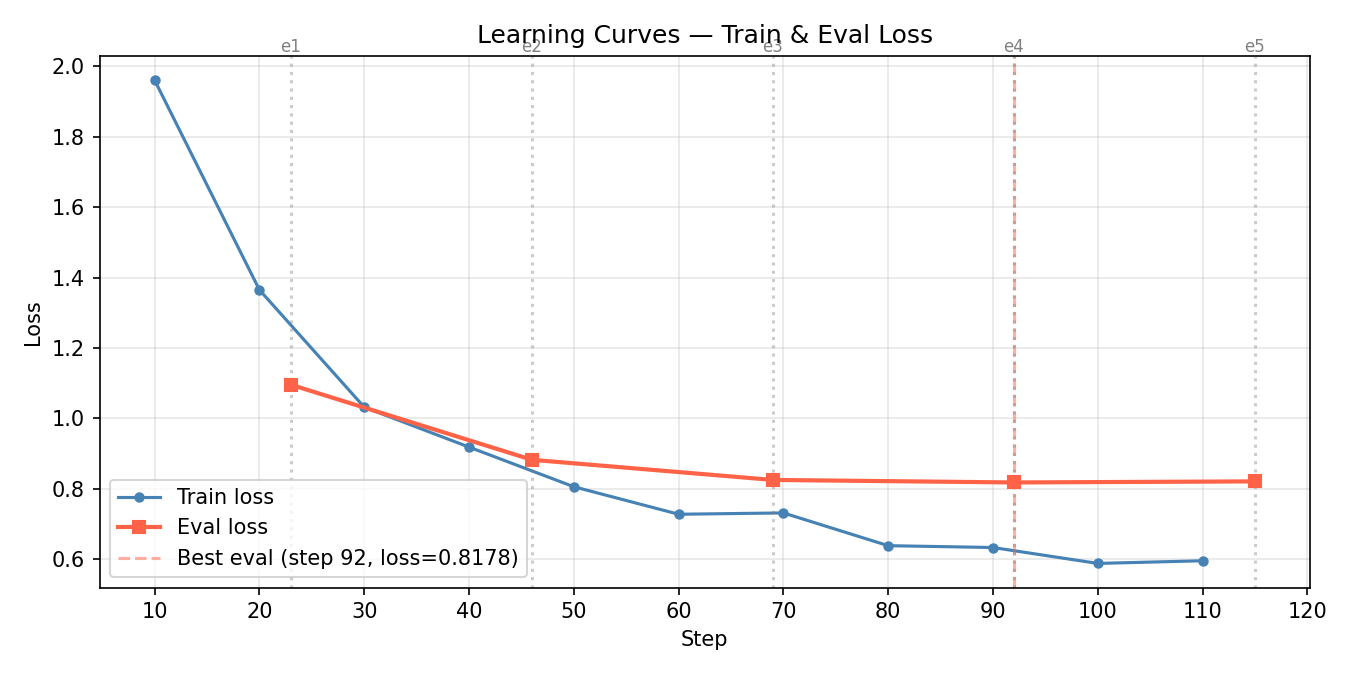
\includegraphics[width=\columnwidth]{img/finetune/deepseek/training_loss_curve.png}
  \caption{Curve di loss per il fine-tuning di DeepSeek-LLM 7B. In blu la training loss per step; in arancione la validation loss valutata al termine di ciascuna epoca. La linea tratteggiata indica il miglior checkpoint (step 92, eval loss $= 0.818$).}
  \label{fig:deepseek_loss}
\end{figure}

Come si osserva in Figura~\ref{fig:deepseek_loss}, la training loss parte da un valore di $1.961$ allo step~10 e decresce in modo regolare fino a $0.595$ al termine dell'addestramento, con la discesa più ripida concentrata nelle prime due epoche. La validation loss, valutata a ogni fine epoca, cala da $1.095$ (epoca~1) a $0.882$ (epoca~2), $0.825$ (epoca~3) e $0.818$ (epoca~4), per poi risalire leggermente a $0.821$ all'epoca~5. Il miglior checkpoint corrisponde quindi allo step~92 (fine epoca~4): anche in questo caso si può notare overfitting, analogo a quanto osservato per Qwen3.5 ma che in questo caso si manifesta leggermente più tardi.

Confrontando i risultati, la validation loss minima di DeepSeek-LLM 7B ($0.818$) è superiore a quella di Qwen3.5-4B ($0.749$). La norma del gradiente si mantiene in un intervallo ristretto $[0.30,\, 0.46]$, sensibilmente più basso rispetto a Qwen3.5, indicando un training stabile e privo di picchi anomali nonostante la quantizzazione. Il profilo del learning rate segue fedelmente lo scheduler coseno atteso, decrescendo da $2 \times 10^{-4}$ fino a valori prossimi a zero nell'ultimo step.

\section{Reinforcement Learning}

Il fine-tuning supervisionato consente ai modelli di apprendere la distribuzione del codice VGDL osservato nel training set, ma ottimizza esclusivamente una loss token-level. Questo significa che il modello viene premiato quando predice sequenze simili al riferimento, senza ricevere un segnale diretto sulla propriet\`a pi\`u importante per il task: la generazione di codice VGDL effettivamente eseguibile e coerente con la descrizione del gioco. Per questo motivo, nella fase successiva si introduce un raffinamento tramite Reinforcement Learning, con l'obiettivo di allineare il comportamento generativo a criteri strutturali e funzionali espliciti.

\subsection{Algoritmo e Setup Sperimentale}

L'ottimizzazione RL \`e stata implementata tramite Group Relative Policy Optimization (GRPO) \citep{shao2024deepseekmath}, una variante di policy optimization adatta al training di LLM perch\'e evita l'uso di un value model separato. Per ciascun prompt, il modello genera un gruppo di completions; ogni completion viene valutata tramite una funzione di reward composita e il vantaggio relativo viene calcolato rispetto alla media del gruppo. In questo modo il modello viene aggiornato per aumentare la probabilit\`a degli output migliori all'interno dello stesso contesto di generazione.

Gli esperimenti RL partono dai checkpoint ottenuti tramite SFT. Il modello base rimane quantizzato a 4 bit e congelato, mentre vengono aggiornati solo i parametri LoRA. Questa scelta mantiene il training compatibile con una singola GPU consumer e consente di confrontare in modo diretto tre condizioni sperimentali: modello zero-shot, modello dopo SFT e modello dopo RL.

\subsection{Funzione di Reward}

La funzione di reward \`e stata progettata per combinare vincoli sintattici, strutturali e semantici. La componente principale misura l'eseguibilit\`a del VGDL generato tramite il parser di \texttt{py-vgdl}; questa reward assegna il punteggio massimo agli output completamente validi e punteggi intermedi agli output che rispettano solo parte della struttura richiesta. Una seconda componente misura la similarit\`a strutturale con il VGDL target, usando lo stesso schema di Jaccard pesato descritto nel protocollo di valutazione: sprite, interazioni e terminazioni.

Sono inoltre incluse reward ausiliarie per incoraggiare la presenza dei blocchi fondamentali (\texttt{SpriteSet}, \texttt{LevelMapping}, \texttt{InteractionSet}, \texttt{TerminationSet}), l'uso di classi sprite e funzioni di interazione appartenenti all'ontologia VGDL, la correttezza delle condizioni di terminazione e il rispetto del formato richiesto, penalizzando output con markdown o testo esplicativo esterno al codice. La reward totale pu\`o quindi essere interpretata come una misura composita della qualit\`a del VGDL generato: non solo "somiglia" al codice target, ma deve anche rispettare i vincoli minimi necessari per essere eseguito.

\subsection{Modelli Raffinati tramite RL}

Il raffinamento tramite GRPO \`e stato applicato ai modelli selezionati dopo la fase zero-shot e SFT. In particolare, Qwen3.5 e DeepSeek dispongono gi\`a dei risultati sperimentali necessari alla discussione finale. Phi-3.5 viene mantenuto come terzo modello selezionato, ma i risultati RL non sono ancora disponibili al momento della stesura; la relativa sezione viene quindi lasciata come placeholder e sar\`a completata dopo l'esecuzione dell'intera pipeline.

\begin{table}[h]
\centering
\caption{Schema dei risultati RL da completare con le metriche finali sul test set.}
\label{tab:rl_results_placeholder}
\begin{adjustbox}{max width=\columnwidth}
\begin{tabular}{lccc}
\toprule
Modello & Zero-shot & SFT & RL \\
\midrule
Qwen3.5 & da inserire & da inserire & da inserire \\
DeepSeek & da inserire & da inserire & da inserire \\
Phi-3.5 & da inserire & da inserire & esperimento non ancora eseguito \\
\bottomrule
\end{tabular}
\end{adjustbox}
\end{table}

\section{Risultati e Discussione}

La valutazione complessiva deve essere letta su due assi complementari. Il primo \`e l'eseguibilit\`a del codice generato: un modello pu\`o produrre testo apparentemente plausibile, ma un singolo riferimento errato a uno sprite, una classe non prevista dall'ontologia VGDL o una condizione di terminazione malformata sono sufficienti a rendere il gioco non eseguibile. Il secondo asse \`e la similarit\`a strutturale con il target, che misura quanto il codice generato rappresenti effettivamente il gioco descritto e non soltanto un VGDL sintatticamente plausibile.

I risultati zero-shot costituiscono una baseline utile ma mostrano i limiti dei modelli non adattati al dominio. Anche quando il formato generale viene rispettato, i modelli tendono a introdurre classi, parametri o interazioni non presenti nell'ontologia di \texttt{py-vgdl}. Questo comportamento \`e coerente con la natura del task: il VGDL \`e un linguaggio specifico, poco rappresentato nei dati di pre-training e caratterizzato da vincoli formali pi\`u rigidi rispetto al linguaggio naturale.

Il fine-tuning supervisionato migliora la capacit\`a dei modelli di riprodurre la struttura del linguaggio. Le curve di training di Qwen3.5 e DeepSeek mostrano una riduzione netta della loss e un apprendimento rapido delle convenzioni sintattiche principali. Tuttavia, la sola riduzione della loss non garantisce eseguibilit\`a: il modello pu\`o imparare pattern frequenti del dataset senza rispettare sempre le dipendenze logiche tra sprite, interazioni e terminazioni. Questo punto \`e particolarmente importante perch\'e nel VGDL la correttezza \`e globale: una definizione mancante nel \texttt{SpriteSet} pu\`o invalidare un'interazione che, localmente, appare ben formata.

Il reinforcement learning affronta precisamente questa debolezza. Inserendo nel processo di ottimizzazione una reward basata su parser, similarit\`a e controlli strutturali, il modello riceve un feedback pi\`u vicino all'obiettivo reale del progetto. I risultati preliminari indicano che il segnale di reward riesce a guidare il modello verso output pi\`u ordinati e pi\`u aderenti ai vincoli del linguaggio, ma mostrano anche una forte variabilit\`a tra step. Questa variabilit\`a \`e attesa: durante GRPO il modello esplora pi\`u completions per prompt e la reward dipende da propriet\`a discrete, come il successo o fallimento del parsing, che possono cambiare bruscamente anche per piccole differenze testuali.

Nel confronto finale tra zero-shot, SFT e RL sar\`a quindi importante non limitarsi alla metrica aggregata media. Sar\`a utile distinguere almeno tre casi: output non eseguibili, output eseguibili ma semanticamente lontani dal target, e output sia eseguibili sia strutturalmente simili al riferimento. Quest'ultima categoria rappresenta il vero obiettivo del progetto. Per Qwen3.5 e DeepSeek, i risultati gi\`a presenti nella repository dovranno essere riportati in una tabella comparativa unica; per Phi-3.5 la stessa analisi verr\`a aggiunta non appena saranno completati SFT, RL e valutazione sul test set.

\section{Limiti}

Il progetto presenta alcuni limiti rilevanti. In primo luogo, il dataset contiene 201 esempi, una dimensione sufficiente per un primo studio esplorativo ma ridotta rispetto agli standard del training di LLM. Questo rende il fine-tuning sensibile all'overfitting e limita la capacit\`a di generalizzazione verso giochi con meccaniche molto diverse da quelle osservate.

In secondo luogo, la similarit\`a strutturale basata su Jaccard cattura componenti importanti del VGDL, ma non misura direttamente la qualit\`a del gameplay prodotto. Due giochi possono condividere sprite e interazioni simili ma produrre dinamiche differenti a seconda della disposizione del livello, delle velocit\`a e dei parametri numerici. Una valutazione pi\`u completa dovrebbe includere simulazioni automatiche o agenti di gioco in grado di testare il comportamento dinamico degli ambienti generati.

Infine, la progettazione della reward introduce un compromesso: reward troppo semplici producono segnali deboli, mentre reward troppo dettagliate rischiano di guidare il modello verso euristiche superficiali. La funzione adottata rappresenta un primo bilanciamento tra eseguibilit\`a, similarit\`a e formato, ma futuri esperimenti potrebbero analizzare separatamente il contributo di ciascuna componente tramite ablation study.

\section{Conclusioni}

Questo lavoro ha presentato una pipeline per la generazione automatica di codice VGDL a partire da descrizioni in linguaggio naturale tramite Large Language Model. A partire dalla costruzione di un dataset dedicato, sono state confrontate tre strategie progressive: prompting zero-shot, fine-tuning supervisionato tramite QLoRA e raffinamento tramite Reinforcement Learning.

I risultati ottenuti mostrano che il fine-tuning supervisionato \`e efficace nell'insegnare ai modelli la struttura superficiale del VGDL, mentre il reinforcement learning consente di introdurre nel processo di ottimizzazione criteri pi\`u vicini alla qualit\`a funzionale del codice generato. La combinazione di parser-based reward e similarit\`a strutturale rappresenta quindi una direzione promettente per domini in cui la correttezza formale \`e essenziale.

Il completamento degli esperimenti su Phi-3.5 e l'integrazione dei risultati finali permetteranno di consolidare il confronto tra modelli e di valutare con maggiore precisione quanto architettura, dimensione e adattamento al dominio incidano sulla generazione di giochi VGDL eseguibili.

\newpage
%% Bibliography
\bibliographystyle{elsarticle-num}
\bibliography{bibliografia}

\end{document}
